\documentclass[12pt, twoside]{article}
\usepackage[letterpaper, margin=1in, headsep=0.5in]{geometry}
\usepackage[english]{babel}
\usepackage[utf8]{inputenc}
\usepackage{amsmath}
\usepackage{amsfonts}
\usepackage{amssymb}
\usepackage{tikz}
\usepackage{yhmath}
%\usetikzlibrary{quotes, angles}

\usepackage{graphicx}
\usepackage{enumitem}
\usepackage{multicol}

\usepackage{fancyhdr}
\pagestyle{fancy}
\fancyhf{}
\renewcommand{\headrulewidth}{0pt} % disable the underline of the header

\fancyhead[RE]{\thepage}
\fancyhead[RO]{\thepage \\ Name: \hspace{3cm}}
\fancyhead[L]{BECA / Dr. Huson / 10th Grade Geometry\\* 7 February 2020}

\begin{document}
\subsubsection*{8.9 Classwork: The equation for a circle}
 \begin{enumerate}%[itemsep=1.5cm]

  \item What is the equation of a circle with center $(5,7)$ and radius $r=3$? \vspace{1cm}

  \item What are the coordinates of the center and the length of the radius of the circle whose equation is $(x-3)^2+y^2=16$? \vspace{1cm}

  \item What is the equation of a circle with center $(-3,7)$ and radius $r=4$?\vspace{1cm}
  
  \item %June 2019
  The equation of a cirle is $x^2+8x+y^2-12y=144$. What are the coordinates of the center and the length of the radius of the circle?
    \begin{enumerate}
      \item center $(4,-6)$ and radius 12
      \item center $(-4,6)$ and radius 12
      \item center $(4,-6)$ and radius 14
      \item center $(-4,6)$ and radius 14
    \end{enumerate}

  \item %June 2018
  What is an equation of circle O shown in the graph below?
  \begin{center}
    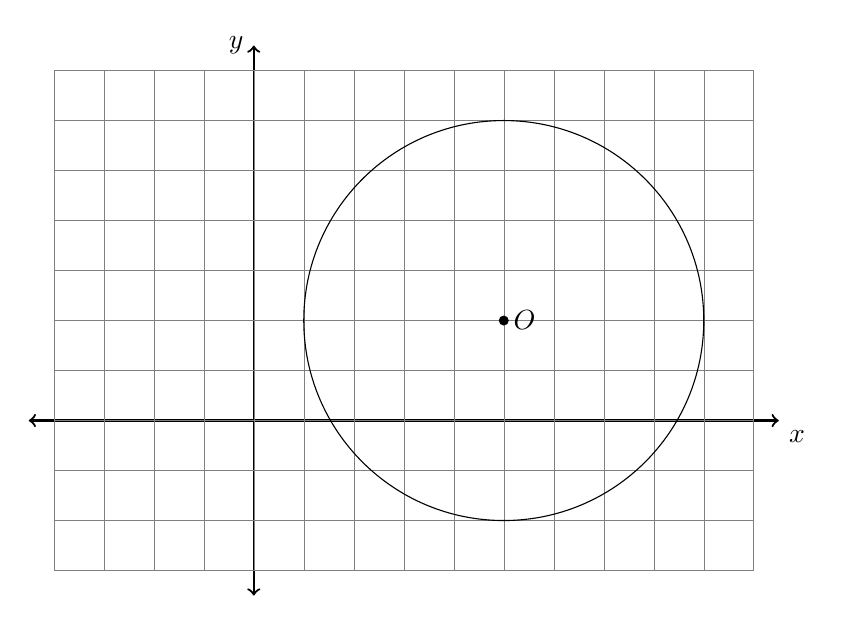
\begin{tikzpicture}[scale=.635]
      \draw [thick, <->] (-4.5,0) -- (10.5,0) node [below right] {$x$};
      \draw [thick, <->] (0,-3.5)--(0,7.5) node [left] {$y$};
      \draw [help lines] (-4,-3) grid (10,7);
      \draw (5,2) circle[radius=4];
        \fill (5,2) circle[radius=.1]node[right]{$O$};
    \end{tikzpicture}
  \end{center}
  \begin{multicols}{2}
    \begin{enumerate}
      \item $x^2+10x+y^2+4y=-13$
      \item $x^2-10x+y^2-4y=-13$
      \item $x^2+10x+y^2+4y=-25$
      \item $x^2-10x+y^2-4y=-25$
    \end{enumerate}
  \end{multicols}

\newpage
  \item %August 2019
  What are the coordinates of the center and the length of the radius of the circle whose equation is $x^2+y^2=8x-6y+39$?
    \begin{enumerate}
      \item center $(-4,3)$ and radius 64
      \item center $(4,-3)$ and radius 64
      \item center $(-4,3)$ and radius 8
      \item center $(4,-3)$ and radius 8
    \end{enumerate}

\item %Jan 2019
What is an equation of a circle whose center is (1,4) and diameter is 10?
  \begin{enumerate}
    \item $x^2-2x+y^2-8y=8$
    \item $x^2+2x+y^2+8y=8$
    \item $x^2-2x+y^2-8y=83$
    \item $x^2+2x+y^2+8y=83$
  \end{enumerate}    
     
  \item %August 2018
  The equation of a cirle is $x^2+y^2+4x-8y=-16$. The statement that best describes circle $O$ is the
    \begin{enumerate}
      \item center is $(2,-4)$ and is tangent to the $x$-axis
      \item center is $(2,-4)$ and is tangent to the $y$-axis
      \item center is $(-2,4)$ and is tangent to the $x$-axis
      \item center is $(-2,4)$ and is tangent to the $y$-axis
    \end{enumerate}

  \item What is the equation of a circle whose diameter is $\overline{AB}$ with $A(2,-1)$ and $B(8,7)$?
    \begin{flushright}
      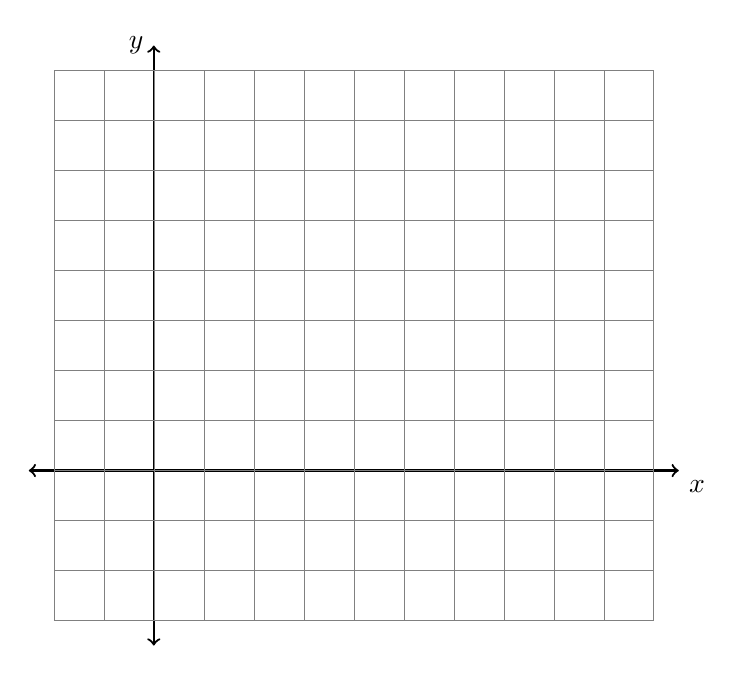
\begin{tikzpicture}[scale=.635]
        \draw [thick, <->] (-2.5,0) -- (10.5,0) node [below right] {$x$};
        \draw [thick, <->] (0,-3.5)--(0,8.5) node [left] {$y$};
        \draw [help lines] (-2,-3) grid (10,8);
          %\draw (5,3) circle[radius=5];
          %\fill (5,3) circle[radius=.1]node[right]{$O$};
          %\draw (2,-1) --(8,7);
      \end{tikzpicture}
    \end{flushright}

\newpage
\subsubsection*{8.9 Exit Note: The equation for a circle}
  \item What are the coordinates of the center and the length of the radius of the circle whose equation is $(x+8)^2+(y-3)^2=4$? \vspace{1.5cm}

  \item What is the equation of a circle with center $(1,-9)$ and radius $r=8$?\vspace{1.5cm}
  
\item What is an equation of circle O shown in the graph below?
  \begin{center}
    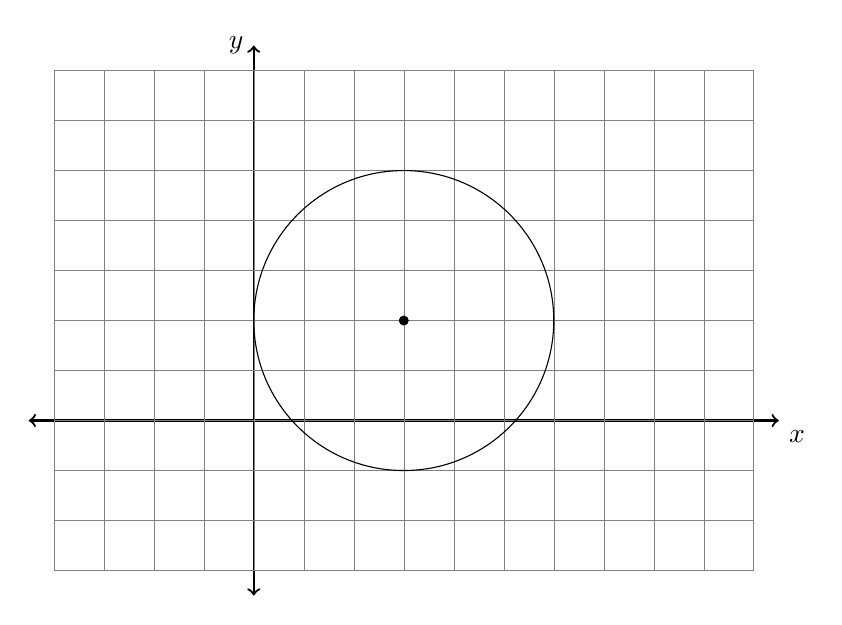
\begin{tikzpicture}[scale=.635]
      \draw [thick, <->] (-4.5,0) -- (10.5,0) node [below right] {$x$};
      \draw [thick, <->] (0,-3.5)--(0,7.5) node [left] {$y$};
      \draw [help lines] (-4,-3) grid (10,7);
      \draw (3,2) circle[radius=3];
        \fill (3,2) circle[radius=.1];
    \end{tikzpicture}
  \end{center} \vspace{2cm}

\item %January 2018
The equation of a cirle is $x^2+y^2-6x+2y=6$. What are the coordinates of the center and the length of the radius of the circle?
  \begin{enumerate}
    \item center $(-3,1)$ and radius 4
    \item center $(3,-1)$ and radius 4
    \item center $(-3,1)$ and radius 16
    \item center $(3,-1)$ and radius 16
  \end{enumerate}

\end{enumerate}
\end{document}
